\begin{enumerate}

\item There are 3 operations used in basic algebra (addition, 
multiplication and exponentiation) and thus
there are potentially 6 different distributive laws.  State
all 6 ``laws'' and determine which 2 are actually valid.
(As an example, the distributive law of addition over multiplication
would look like $x + (y \cdot z) = (x + y) \cdot (x + z)$, this isn't 
one of the true ones.) 

\wbvfill

\hint{
\vfill

These ``laws'' should probably be layed-out in a big 3 by 3 table. Such a table would of course have 9 cells, but we won't be using the cells on the diagonal because they would involve an operation distributing over itself. (That can't happen, can it?)
I'm going to put a few of the entries in, and you do the rest.

\vfill

\begin{tabular}{c|c|c|c|} 
  & \rule{36pt}{0pt} $+$ \rule{36pt}{0pt} & \rule{36pt}{0pt} $\ast$ \rule{36pt}{0pt} & \rule{36pt}{0pt} $\caret$ \rule{36pt}{0pt} \\ \hline
 \rule[-36pt]{0pt}{72pt} $+$ & $\emptyset$ & \parbox{1.4in}{\begin{gather*}x+(y\ast z) \\= (x+y) \ast (x+z)\end{gather*}} & \parbox{1.4in}{\begin{gather*}x+(y^z) \\ = (x+y)^{(x+z)} \end{gather*} } \\ \hline
 \rule[-36pt]{0pt}{72pt} $\ast$ & \parbox{1.4in}{\begin{gather*} x \ast (y+z) \\ = (x \ast y) + (x \ast z)\end{gather*} } & $\emptyset$ &  \\ \hline
 \rule[-36pt]{0pt}{72pt} $\caret$ & & & $\emptyset$ \\ \hline
\end{tabular}

\vfill

\rule{0pt}{0pt}
 }
 
 \workbookpagebreak
\hintspagebreak
 
\item Use truth tables to verify or disprove the following 
logical equivalences.

\begin{enumerate}
\item $(A \land B) \lor B \; \cong \; (A \lor B) \land B$
\item $A \land (B \lor {\lnot}A) \; \cong \; A \land B $
\item $(A \land {\lnot}B) \lor ({\lnot}A \land {\lnot}B) \cong
(A \lor {\lnot}B) \land ({\lnot}A \lor {\lnot}B)$ 
\item The absorption laws.
\end{enumerate}

\wbvfill

\hint{You should be able to do these on your own.}

\workbookpagebreak

\item Draw pairs of related digital logic circuits that illustrate
DeMorgan's laws.

\wbvfill

\hint{
Here's the pair that shows the negation of an AND is the same as the OR of the same inputs negated.

\centerline{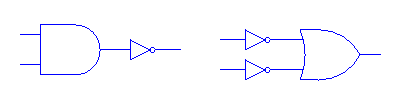
\includegraphics{figures/DeMorgan}}
}

\item Find the negation of each of the following and simplify as much as possible.
\medskip

  \begin{enumerate}
  \item $(A \lor B) \; \iff \; C$
\medskip

  \item $(A \lor B) \; \implies \; (A \land B)$

  \end{enumerate}

\wbvfill

\hint{Neither of these is particularly amenable to simplification. Nor, perhaps, is it readily
apparent what ``simplify'' means in this context! My interpretation is that we should look
for a logically equivalent expression using the fewest number of operators and if possible
{\em not} using the more complicated operators ($\implies$ and $\iff$).  However, if we try 
to rewrite the first statement's negation using only $\land$, $\lor$ and $\lnot$ we get things
that look a lot more complicated than $(A \lor B) \; \iff \; {\lnot}C$ -- the quick way to negate a 
bicondiitonal is simply to negate one of its parts.

The second statement's negation turns out to be the same thing as exclusive or, so a particularly
simple response would be to write $A \oplus B$ although that feels a bit like cheating, so
maybe we should answer with $(A \lor B) \land {\lnot}(A \land B)$ -- but that answer is what we
would get by simply applying the rule for negating a conditional and doing no further simplification.
}

\workbookpagebreak

\item Because a conditional sentence is equivalent to a certain disjunction, and 
because DeMorgan's law tells us that the negation of a disjunction is a conjunction,
it follows that the negation of a conditional is a conjunction.  Find denials (the negation
of a sentence is often called its ``denial'') for each of the following conditionals.

\begin{enumerate}
\item ``If you smoke, you'll get lung cancer.''
\item ``If a substance glitters, it is not necessarily gold.''
\item ``If there is smoke, there must also be fire.''
\item ``If a number is squared, the result is positive.''
\item ``If a matrix is square, it is invertible.''
\end{enumerate}

\wbvfill

\hint{
\begin{enumerate}
\item ``You smoke and you haven't got lung cancer.''
\item ``A substance glitters and it is necessarily gold.''
\item ``There is smoke,and there isn't fire.''
\item ``A number is squared, and the result is not positive.''
\item ``A matrix is square and it is not invertible.''
\end{enumerate}
}

\hintspagebreak
\workbookpagebreak

\item The so-called ``ethic of reciprocity'' is an idea that has come 
up in many of the world's religions and philosophies.  
Below are statements of the ethic
from several sources.  Discuss their logical meanings and determine which (if 
any) are logically equivalent.

\begin{enumerate}
\item ``One should not behave towards others in a way which is disagreeable to oneself.'' Mencius Vii.A.4 (Hinduism)
\item ``None of you [truly] believes until he wishes for his brother what he wishes for himself.'' Number 13 of Imam ``Al-Nawawi's Forty Hadiths.'' (Islam)
\item ``And as ye would that men should do to you, do ye also to them likewise.'' Luke 6:31, King James Version. (Christianity)
\item ``What is hateful to you, do not to your fellow man. This is the law: all the rest is commentary.'' Talmud, Shabbat 31a. (Judaism)
\item ``An it harm no one, do what thou wilt'' (Wicca)
\item ``What you would avoid suffering yourself, seek not to impose on others.'' (the Greek philosopher Epictetus -- first century A.D.)
\item ``Do not do unto others as you expect they should do unto you. Their tastes may not be the same.'' (the Irish playwright George Bernard Shaw -- 20th century A.D.)
\end{enumerate}

\wbvfill

\hint{
The ones from Wicca and George Bernard Shaw are just there for laughs.

For the remainder, you may want to contrast how restrictive they seem. For example the Christian version is (in my opinion) a lot stronger than the one from the Talmud -- ``treat others as you would want to be treated'' restricts your actions both in terms of what you would like done to you and in terms of what you wouldn't like done to you; ``Don't treat your fellows in a way that would be hateful to you.'' is leaving you a lot more freedom of action, since it only prohibits you from doing those things you wouldn't want done to yourself to others. The Hindus, Epictetus and the Jews (and the Wiccans for that matter) seem to be expressing roughly the same sentiment -- and promoting an ethic that is rather more easy for humans to conform to!

From a logical perspective it might be nice to define open sentences:

\[ W(x,y) \; = \; \mbox{``x would want y done to him.''} \]

\[ N(x,y)  \; = \; \mbox{``x would not want y done to him.''} \]

\[ D(x,y)  \; = \; \mbox{``do y to x.''} \]

\[ DD(x,y)  \; = \; \mbox{``don't do y to x.''} \]

In which case, the aphorism from Luke would be

\[ (W(you, y) \implies  D(others, y)) \land (N(you, y) \implies DD(others, y)) \]

}

\workbookpagebreak
\textbookpagebreak

\item You encounter two natives of the land of knights and knaves. Fill
in an explanation for each line of the proofs of their identities. 

\begin{enumerate}
\item Natasha says, ``Boris is a knave.'' \\
Boris says, ``Natasha and I are knights.''\\

\hintspagebreak

\textbf{Claim:} Natasha is a knight, and Boris is a knave.\\

\begin{proof} If Natasha is a knave, then Boris is a knight.\\
If Boris is a knight, then Natasha is a knight.\\
Therefore, if Natasha is a knave, then Natasha is a knight.\\
Hence Natasha is a knight.\\
Therefore, Boris is a knave.
\end{proof}

\item Bonaparte says ``I am a knight and Wellington is a knave.''\\
Wellington says ``I would tell you that B is a knight.''

\textbf{Claim:} Bonaparte is a knight and Wellington is a knave.

\begin{proof}
    Either Wellington is a knave or Wellington is a knight.\\
    If Wellington is a knight it follows that Bonaparte is a knight.\\
    If Bonaparte is a knight then Wellington is a knave. \\
    So, if Wellington is a knight then Wellington is a knave (which is impossible!)\\
    Thus, Wellington is a knave.\\
    Since Wellington is a knave, his statement ``I would tell you that Bonaparte is a knight'' is false. \\
    So Wellington would in fact tell us that Bonaparte is a knave. \\
    Since Wellington is a knave we conclude that Bonaparte is a knight.\\
    Thus Bonaparte is a knight and Wellington is a knave (as claimed).\\
\end{proof}

\hintspagebreak
\wbvfill

\hint{
Here's the second one:

\begin{proof}
    Either Wellington is a knave or Wellington is a knight.\\
    \rule{0pt}{0pt} \hfill \parbox{3in}{\color[rgb]{1,0,0} It's either one thing or the other! }\\
    If Wellington is a knight it follows that Bonaparte is a knight.\\
    \rule{0pt}{0pt} \hfill \parbox{3in}{\color[rgb]{1,0,0} That's what he said he would tell us and if he's a knight we can trust him.}\\
    If Bonaparte is a knight then Wellington is a knave. \\
    \rule{0pt}{0pt} \hfill \parbox{3in}{\color[rgb]{1,0,0} True, because that is one of the things Bonaparte states.}\\
    So, if Wellington is a knight then Wellington is a knave (which is impossible!)\\
    \rule{0pt}{0pt} \hfill \parbox{3in}{\color[rgb]{1,0,0} This is just summing up what was deduced above.}\\
    Thus, Wellington is a knave.\\
    \rule{0pt}{0pt} \hfill \parbox{3in}{\color[rgb]{1,0,0}  Because the other possibility leads to something {\em im}possible.}\\
    Since Wellington is a knave, his statement ``I would tell you that Bonaparte is a knight'' is false. \\
    \rule{0pt}{0pt} \hfill \parbox{3in}{\color[rgb]{1,0,0} Knave's statements are always false!}\\
    So Wellington would in fact tell us that Bonaparte is a knave. \\
    \rule{0pt}{0pt} \hfill \parbox{3in}{\color[rgb]{1,0,0} He was lying when he said he would tell us B is a knight.} \\
    Since Wellington is a knave we conclude that Bonaparte is a knight.\\
    \rule{0pt}{0pt} \hfill \parbox{3in}{\color[rgb]{1,0,0} Wait, now I'm confused\ldots can you do this part?} \\
    Thus Bonaparte is a knight and Wellington is a knave (as claimed).\\
    \rule{0pt}{0pt} \hfill \parbox{3in}{\color[rgb]{1,0,0} Just summarizing.} \\
\end{proof}

}

\end{enumerate}

\end{enumerate}
